''Four rollers mill'' flow driven by body force defined by
\begin{align*}
  f_x &= A \sin \overline{x} \cos \overline{y}, \\
  f_y &= A \cos \overline{x} \sin \overline{y}
\end{align*}
where $A$ is the force amplitude, $\overline{x} = 2 \pi x / L$,
$\overline{y} = 2 \pi y / L$. Two cases are considered with only
difference in the viscosity ratios: $\lambda \approx \mu_{inside} /
\mu_{outside}$. ``More viscous'' RBCs tend to stay away from high
shear regions.

\begin{figure}
\begin{center}
  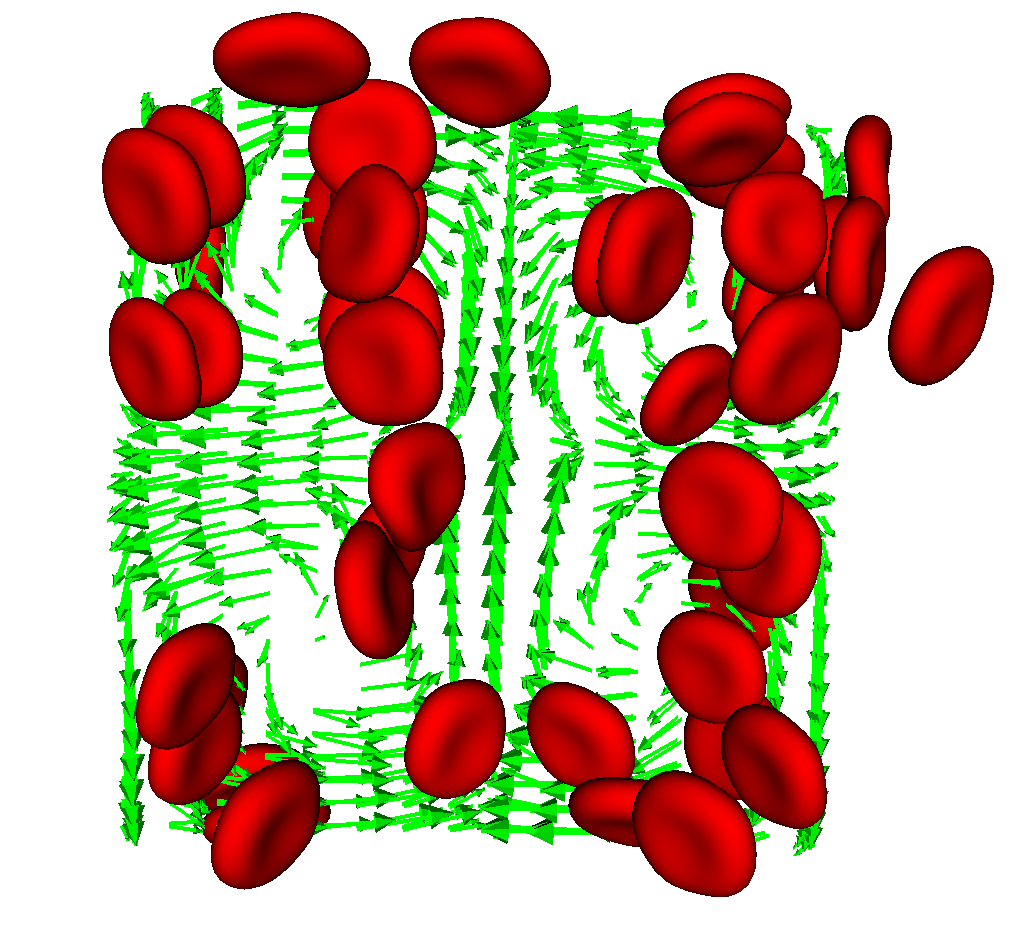
\includegraphics[width=0.4\textwidth]{i/rbc/a/visit.png}
  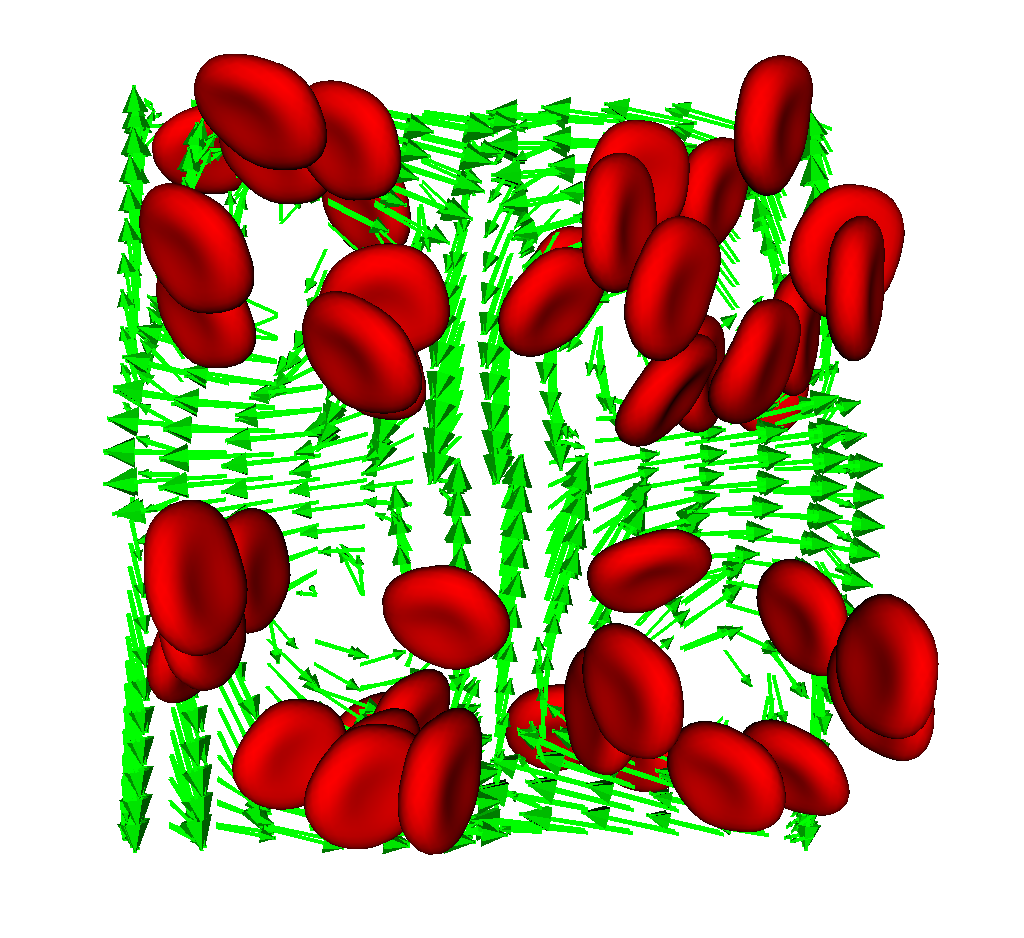
\includegraphics[width=0.4\textwidth]{i/rbc/b/visit.png}
  \caption{Left $\lambda = 100$, right $\lambda = 1$}
\end{center}
\end{figure}
